\chapter{Simulation Environment and Experimental Setup}
\section{Role of Simulation in the Thesis}
The development of the ACTS requires the interaction of several coupled mechanical and control components. A physics-based simulation environment is therefore used to evaluate the proposed architectures and control strategies before physical implementation.

Simulation provides a controlled environment in which the system can be tested under repeatable conditions. It also enables the evaluation of the controller without the risks and practical constraints associated with experiments on a physical system.

An additional advantage of using a physics engine is that the complete coupled equations of motion do not need to be explicitly derived and numerically integrated for each configuration. Instead, the mechanical bodies, joints, constraints, actuators, and contact properties are defined in the simulation model, while the physics engine performs the corresponding numerical integration. Nevertheless, the validity of the simulation remains dependent on the assumptions and simplifications made in the model.

\section{Simulator Selection}

Two simulation environments were investigated during the development of the thesis: Gazebo and MuJoCo. Gazebo was initially considered because of its integration with ROS2 and the availability of existing UAV models and visualization tools. However, difficulties were encountered when attempting to represent the closed cable-constrained structure of the ACTS. MuJoCo was therefore selected for the final simulation environment.

\subsection{Gazebo Environment}
Gazebo Harmonic \cite{gazebo_harmonic_getstarted} was initially selected as a potential simulation environment because of its established use in robotics and its integration with ROS2. However, the ACTS architecture presents a particular modeling challenge. Indeed, Gazebo assigns each physical element in the simulation a parent, generating a tree-like structure. While this does not constitute a problem for conventional articulated robot, ACTS contains ground cables constrained at both ends (resp. on the payload and on a point fixed on the ground), resulting in closed kinematic constraints. 

Additionally, cables as soft body cannot be modelled in Gazebo, as it only manage rigid object. To go around the problem, they are modelled using multiple rigid links connected using universal joints. Although it solved the problem, implementing it resulted into an impracticable slow-down simulation.

Several preliminary simulations were nevertheless successfully implemented in Gazebo, including a pulley mechanism, a UAV connected to the ground through a cable, and a UAV connected to a payload. While individual components of the system could be simulated, such as pulley mechanism and single drone-cable simulation, extending this approach to the complete ACTS resulted in a more complex and computationally demanding model.

These experiments were useful for validating the initial modeling approach and identifying the main limitations before transitioning to another simulation environment.

\todo[inline]{Add photos?}

Given the additional modeling effort required to represent the complete ACTS architecture and the limited time available for the thesis, continuing the Gazebo implementation was not considered the most effective approach for obtaining the required simulation results.

\subsection{MuJoCo Environment}

MuJoCo (Multi-Joint dynamics with Contact) was selected as the final simulation environment because it is well suited to the closed-loop structure of cable-driven robots. In particular, MuJoCo provides tendon elements that can be used to represent cable-like connections between bodies, including constraints associated with their geometric configuration \cite{mujoco_docs_237}.

This capability significantly simplifies the representation of the ACTS compared with the rigid-link approximation investigated in Gazebo. The complete system can therefore be represented using the payload, UAVs, ground anchors, and cables while maintaining the closed-loop constraints required by the architecture.

For the simulations presented in this thesis, the cables are modeled as ideal geometric constraints. Their stiffness and damping are neglected, such that the cables transmit tensile forces without introducing additional elastic dynamics. This simplification is consistent with the quasi-static and geometric analysis used for the architecture evaluation, while allowing the simulation to focus on the influence of cable configuration, attachment geometry, and actuator placement.

\section{Software architecture (UML)}
"How did I implement the simulator?"
Figure: UML/software architecture.

Overall Software Architecture \\
Drone Controller Class Hierarchy
\begin{figure}[h]
    \centering
    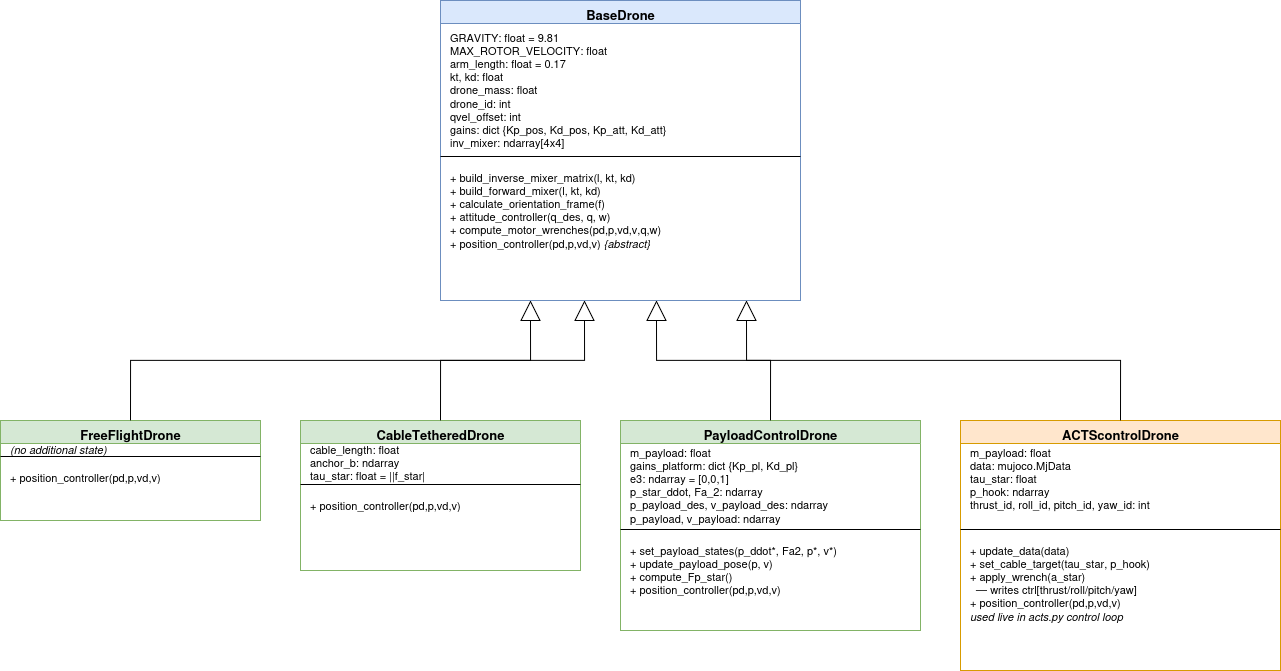
\includegraphics[width=\linewidth]{images/class_diagram.png}
    \caption{Class Diagram}
    \label{fig:classDiagram}
\end{figure}

Simulation and Data Processing Pipeline


Python packages/modules
UML architecture
how the XML-generation code interacts with the simulator
how the MuJoCo API is interfaced with
controller classes
simulation loop
optimization
data collection
performance evaluation software

\section{Simulation setup}
"This is what the simulator contains."

Figures/tables: MuJoCo model + simulation parameters + representative configurations.

Parameter	Value
Number of UAVs	3
Payload mass	...
UAV mass	...
Cable length	...
Simulation timestep	...
Maximum UAV thrust	...
Position tolerance	...
Orientation tolerance	...
Initial payload pose	...
Target payload pose

5.4.1 Simulation model
Describe the actual ACTS instance used in MuJoCo.

For example:
The simulation consists of three UAVs connected to a rigid payload through aerial cables, with additional ground cables connected to fixed anchor points...

You're not explaining how the Python code implements it. You're describing the model itself.

5.4.2 Simulation parameters
Put your numerical parameters in a table.

5.4.3 Initial and target conditions
Initial payload pose, target pose, UAV positions, etc.

5.4.4 Configurations considered
Stewart baseline, different ground routings, hook placements, etc.

\section{Simulation methodology and evaluation framework}

%% Experimental objectives
The objective of this chapter is to evaluate how the architectural design of an ACTS influences its ability to accurately and robustly manipulate a payload. The focus is on how different cable routing strategies, UAV attachment configurations, and ground hook placements influence the overall system performance.

In fact, a configuration is considered successful if the desired payload is reached with sufficiently small position and orientation errors, all cables remain under positive tension throughout the maneuver, and the payload converges to an equilibrium without persistent oscillations.

In the following chapter we will answer questions like "Which configuration gives the best payload control performance according to the theoretical indices?" and "Which configuration would I actually choose for the robot?"

%% Simulation setup.  Why simulate the controller instead of only computing the Jacobian?
The geometric and static performance indices provided in Section \ref{sec:performanceIndices} describe the instantaneous ability of a given architecture to generate payload wrenches and identify configurations that are close to kinematic singularities. However, these indices are evaluated under static or quasi-static assumptions and therefore cannot fully characterize the behavior of the closed-loop system during motion. During motion, cable directions, tensions and payload dynamics continuously evolve. Consequently, a configuration that appears favorable according to static indices may still exhibit oscillations, poor tracking or instability. Closed-loop simulation is therefore necessary to verify whether the theoretical advantages translate into practical performance.


%% Variables
The payload mass, UAV model, controller gains, drone cable lengths, simulation duration, and desired payload pose are kept constant throughout all experiments to ensure a fair comparison between different architectural configurations. The only variables that change from one experiment to another are the cable routing, the UAV attachment geometry, and the placement of the ground hook points.

%% Scenario A and B
Two desired payload poses are taken in considerations. In the first scenario, the desired payload orientation coincides with the world reference frame; while in the other scenario a non-zero desired orientation is imposed. This allows to analyze separately the rotational motions from the translation tracking.

%% Why did you choose Stewart as the reference?
First, the classical Stewart configuration is analyzed and used as a reference architecture due to its geometric symmetry and extensive use in the literature. In fact, if even Stewart-like performs poorly, the problem is likely the controller rather than the architecture. The remaining experiments then investigate how modifications to the ground cable routing, UAV attachment geometry, and hook placement affect both the theoretical performance indices and the closed-loop behavior of the system. This progressive analysis makes it possible to identify which geometric features have the greatest influence on payload manipulation performance.

%%The attachment points are uniformly distributed, which generally leads to good isotropy.